\documentclass{article}

\usepackage{listings}
\usepackage{bbold}
\usepackage{graphicx}
\usepackage[spanish]{babel}
\usepackage[top=3cm,bottom=3cm,left=2cm,right=2cm]{geometry}
\usepackage[utf8]{inputenc}
\usepackage{amsmath,amsfonts,amssymb}
\usepackage{multirow}
\usepackage{booktabs}
\usepackage{caption}
\usepackage{bbold}
\usepackage{fancyhdr}
\usepackage{tikz}



\newcommand{\abs}[1]{ \lvert #1 \rvert }
\newcommand{\sii}{\Leftrightarrow}
\newcommand{\limi}{\liminf_n A_n}
\newcommand{\lims}{\limsup_n A_n}
\newcommand{\then}{\Rightarrow}
\newcommand{\RR}{\mathbb{R}}
\newcommand{\norm}[1]{\lvert \lvert #1 \rvert \rvert}
\newcommand{\prob}{\stackrel{p}{\to}}
\newcommand{\ton}{\stackrel{n}{\to}\,}
\newcommand{\E}{\mathbb{E} \,}
\newcommand{\limn}{\lim_{n\to +\infty}}
\newcommand{\cuadro}[3]{\setbox0\hbox{#1 \hspace{-1em}\raisebox{1em}{$\downarrow$}} \clap{\hbox to \wd0{\raisebox{#2\height}{#3}}}\box0 \;}
\newcommand{\cuadrodos}[3]{\setbox0\hbox{#1}  \llap{\hbox to \wd0{\raisebox{#2\height}{#3}}}\box0 \;}
\newcommand{\cs}{\stackrel{c.s.}{\to}}
\newcommand{\ind}[1]{1\hspace{-0.35em}1_{ \{ #1 \} } }
\newcommand{\mean}[1]{\bar{#1}_n}
\newcommand{\MAS}{$X_1, \dots, X_n$ MAS de $X$ }
\newcommand{\minim}{X_{(1:n)}}
\newcommand{\p}{\mathbb{P}}
\newcommand{\up}[1]{\stackrel{\text{#1}}{=}}
\newcommand{\f}{\mathcal{F}}
\newcommand{\bb}[1]{\bold{#1}}
\newcommand{\prodi}[1]{\left\langle #1 \right\rangle}
%\newcommand{\norm}[1]{\left\langle #1 \right\rangle}

\graphicspath{{/home/manuel/Dropbox/temperaturas/git/dlm_temp/graf/}}


\usepackage{fancyhdr}

\setlength{\parskip}{20pt}
\setlength{\headheight}{15 pt}
\pagestyle{fancy}

\rhead{}
\lhead{}
\rhead{}
\chead{}
\rfoot{}
%\renewcommand{\headrulewidth}{0pt}
\renewcommand{\footrulewidth}{0.5pt}
\newcommand{\HRule}{\rule{\linewidth}{0.5mm}}


\begin{document}


\begin{titlepage}
\begin{center}

% Upper part of the page. The '~' is needed because \\
% only works if a paragraph has started.


\vspace*{\fill}
\textsc{\LARGE Universidad de la República}\\[1.5cm]

\textsc{\Large Facultad de Ciencias Económicas y Administración}\\[1.5cm]

\textsc{\large Instituto de Estadística}\\[1.5cm]


\includegraphics[width=1.25in]{logoiesta.png}~\\[1cm]

\textsc{\large Documento de trabajo}\\[0.5cm]


% Title
\HRule \\[0.4cm]
{\Large \bfseries Detección de olas de frío a través de DLM }

\HRule \\[1.5cm]

% Author and supervisor
\begin{minipage}{0.4\textwidth}
\begin{flushleft}
\emph{Autor:}\\
Manuel \textsc{Hernández Banadik}
\\
\end{flushleft}
\end{minipage}
\begin{minipage}{0.4\textwidth}
\begin{flushright}
\emph{Docentes:} \\
\textit{PhD.} Ignacio \textsc{Álvarez-Castro}
\end{flushright}
\end{minipage}

\vfill

% Bottom of the page
{\large \today}

\end{center}
\end{titlepage}\pagebreak


\tableofcontents
\listoffigures
\listoftables

\begin{abstract}

Contamos con datos de mediciones diarias de temperaturas mínimas y máximas, de una estación meteorológica de Uruguay, desde Enero-1950 a Octubre-2014.

Se define una ola de frío, como un período de tiempo en el cual, la temperatura observada es inferior a un umbral. El objetivo es determinar dicho umbral a través de la estimación del percentil 10 de las temperaturas. Utilizaremos los modelos lineales dinámicos para modelar la serie, y para la estimación de los percentiles.

\end{abstract}

\section{Olas de frío}

Existen diversas formas de caracterizar una racha de frío, que responden a distintas aplicaciones de su estudio. Las diversas definiciones acuerdan en la necesidad de establecer un umbral de bajas temperaturas (puede ser absoluto o relativo) y en delimitar una ventana de tiempo mínimo. Durante ese tiempo, la temperatura observada debe mantenerse siempre por debajo del umbral definido.

Para el presente trabajo, hemos definido una ola de frío como un período de tiempo mayor o igual a 3 días, en los cuales las temperaturas mínimas y máximas son inferiores a los respectivos percentiles 10 esperados para tales días.

Esta definición requiere de definir para cada día del año un percentil 10 de temperatura mínima y máxima. Para cada $t \in \{1,\dots, 365\}$ definimos el percentil 10 de mínima como $p^n_{10_t}:= \inf\{y: \p(Y^n_t \leq y)\geq 0.1\}$ siendo $Y^n_t$ la temperatura mínima observada en el día $t$. Análogamente definimos el percentil 10 de máxima para el día $t$ como $p^x_{10_t}:= \inf\{y: \p(Y^x_t \leq y)\geq 0.1\}$ donde $Y^x_t$ es la temperatura máxima observada en el día $t$.

Podemos decir entonces que una sucesión de días $t_1, \dots, t_k$ constituyen una ola de frío de largo $k$ si, siendo $k\geq 3$, se cumple simultáneamente que:
$\begin{cases} y^n_{t_i} < p^n_{10_i}  \\ y^x_{t_i} < p^x_{10_i} \end{cases}$ para $i=1,\dots,k$

\section{Dynamic Linear Models}

%Los modelos lineales dinámicos (DLM) son una familia de modelos de espacio de estado. Procesos muy conocidos pueden ser vistos como modelos DLM: el paseo al azar, el modelo de regresión normal, los modelos ARIMA, entre otros.
%
%Un modelo estadístico de posición, establece que hay un parámetro del cual tenemos observaciones ruidosas. %Podemos extender esa idea, y considerar que tenemos obervaciones ruidosas de un
%Podemos extender la idea de parámetro 

Un modelo lineal dinámico (DLM) considera una serie de tiempo, como una observación ruidosa de un proceso dinámico. La figura \ref{fig:graf7} muestra un ejemplo de un proceso concebido de esta forma. El modelo está definido a través de una ecuación de evolución y una ecuación de observación. La ecuación de evolución define cómo se vincula el estado del proceso en tiempo $t$ con su estado en tiempo $t+1$; la ecuación de observación, explicita cómo es observado el proceso en tiempo $t$ en función del estado en el que se encuentra a $t$. En una expresión y/o en la otra, se introduce un componente aleatorio.

Tenemos entonces la siguiente expresión para el modelo:
%\begin{center}
%$\begin{array}{lc}
%Y_t=F_t\theta_t + v_t  &  v_t \sim \mathcal{N}(0,V_t) \\
%\theta_t = G_t \theta_{t-1} + w_t \;\; & w_t \sim \mathcal{N}(0,W_t)
%\end{array}$
%\end{center}
\begin{equation}
\begin{aligned}
Y_t&=F_t\theta_t + v_t  \;&\;  v_t \sim \mathcal{N}(0,V_t) \\
\theta_t &= G_t \theta_{t-1} + w_t \;&\; w_t \sim \mathcal{N}(0,W_t)
\end{aligned}
\label{eq:modelo}
\end{equation} donde las matrices $F_t,G_t,V_t,W_t$ serán los parámetros que caractericen el modelo. $\mathcal{N}$ es la distribución normal.

Si se tiene las observaciones $y_1,\dots,y_T$, puede ser de interés obtener una estimación de $\E(\theta_t | y_1,\dots,y_t)$, es decir, el valor esperado del proceso que subyace a las observaciones en tiempo $t$, dado que tenemos las observaciones pasadas. Esta cantidad es estimada mediante el Filtro de Kalman.

\begin{center}
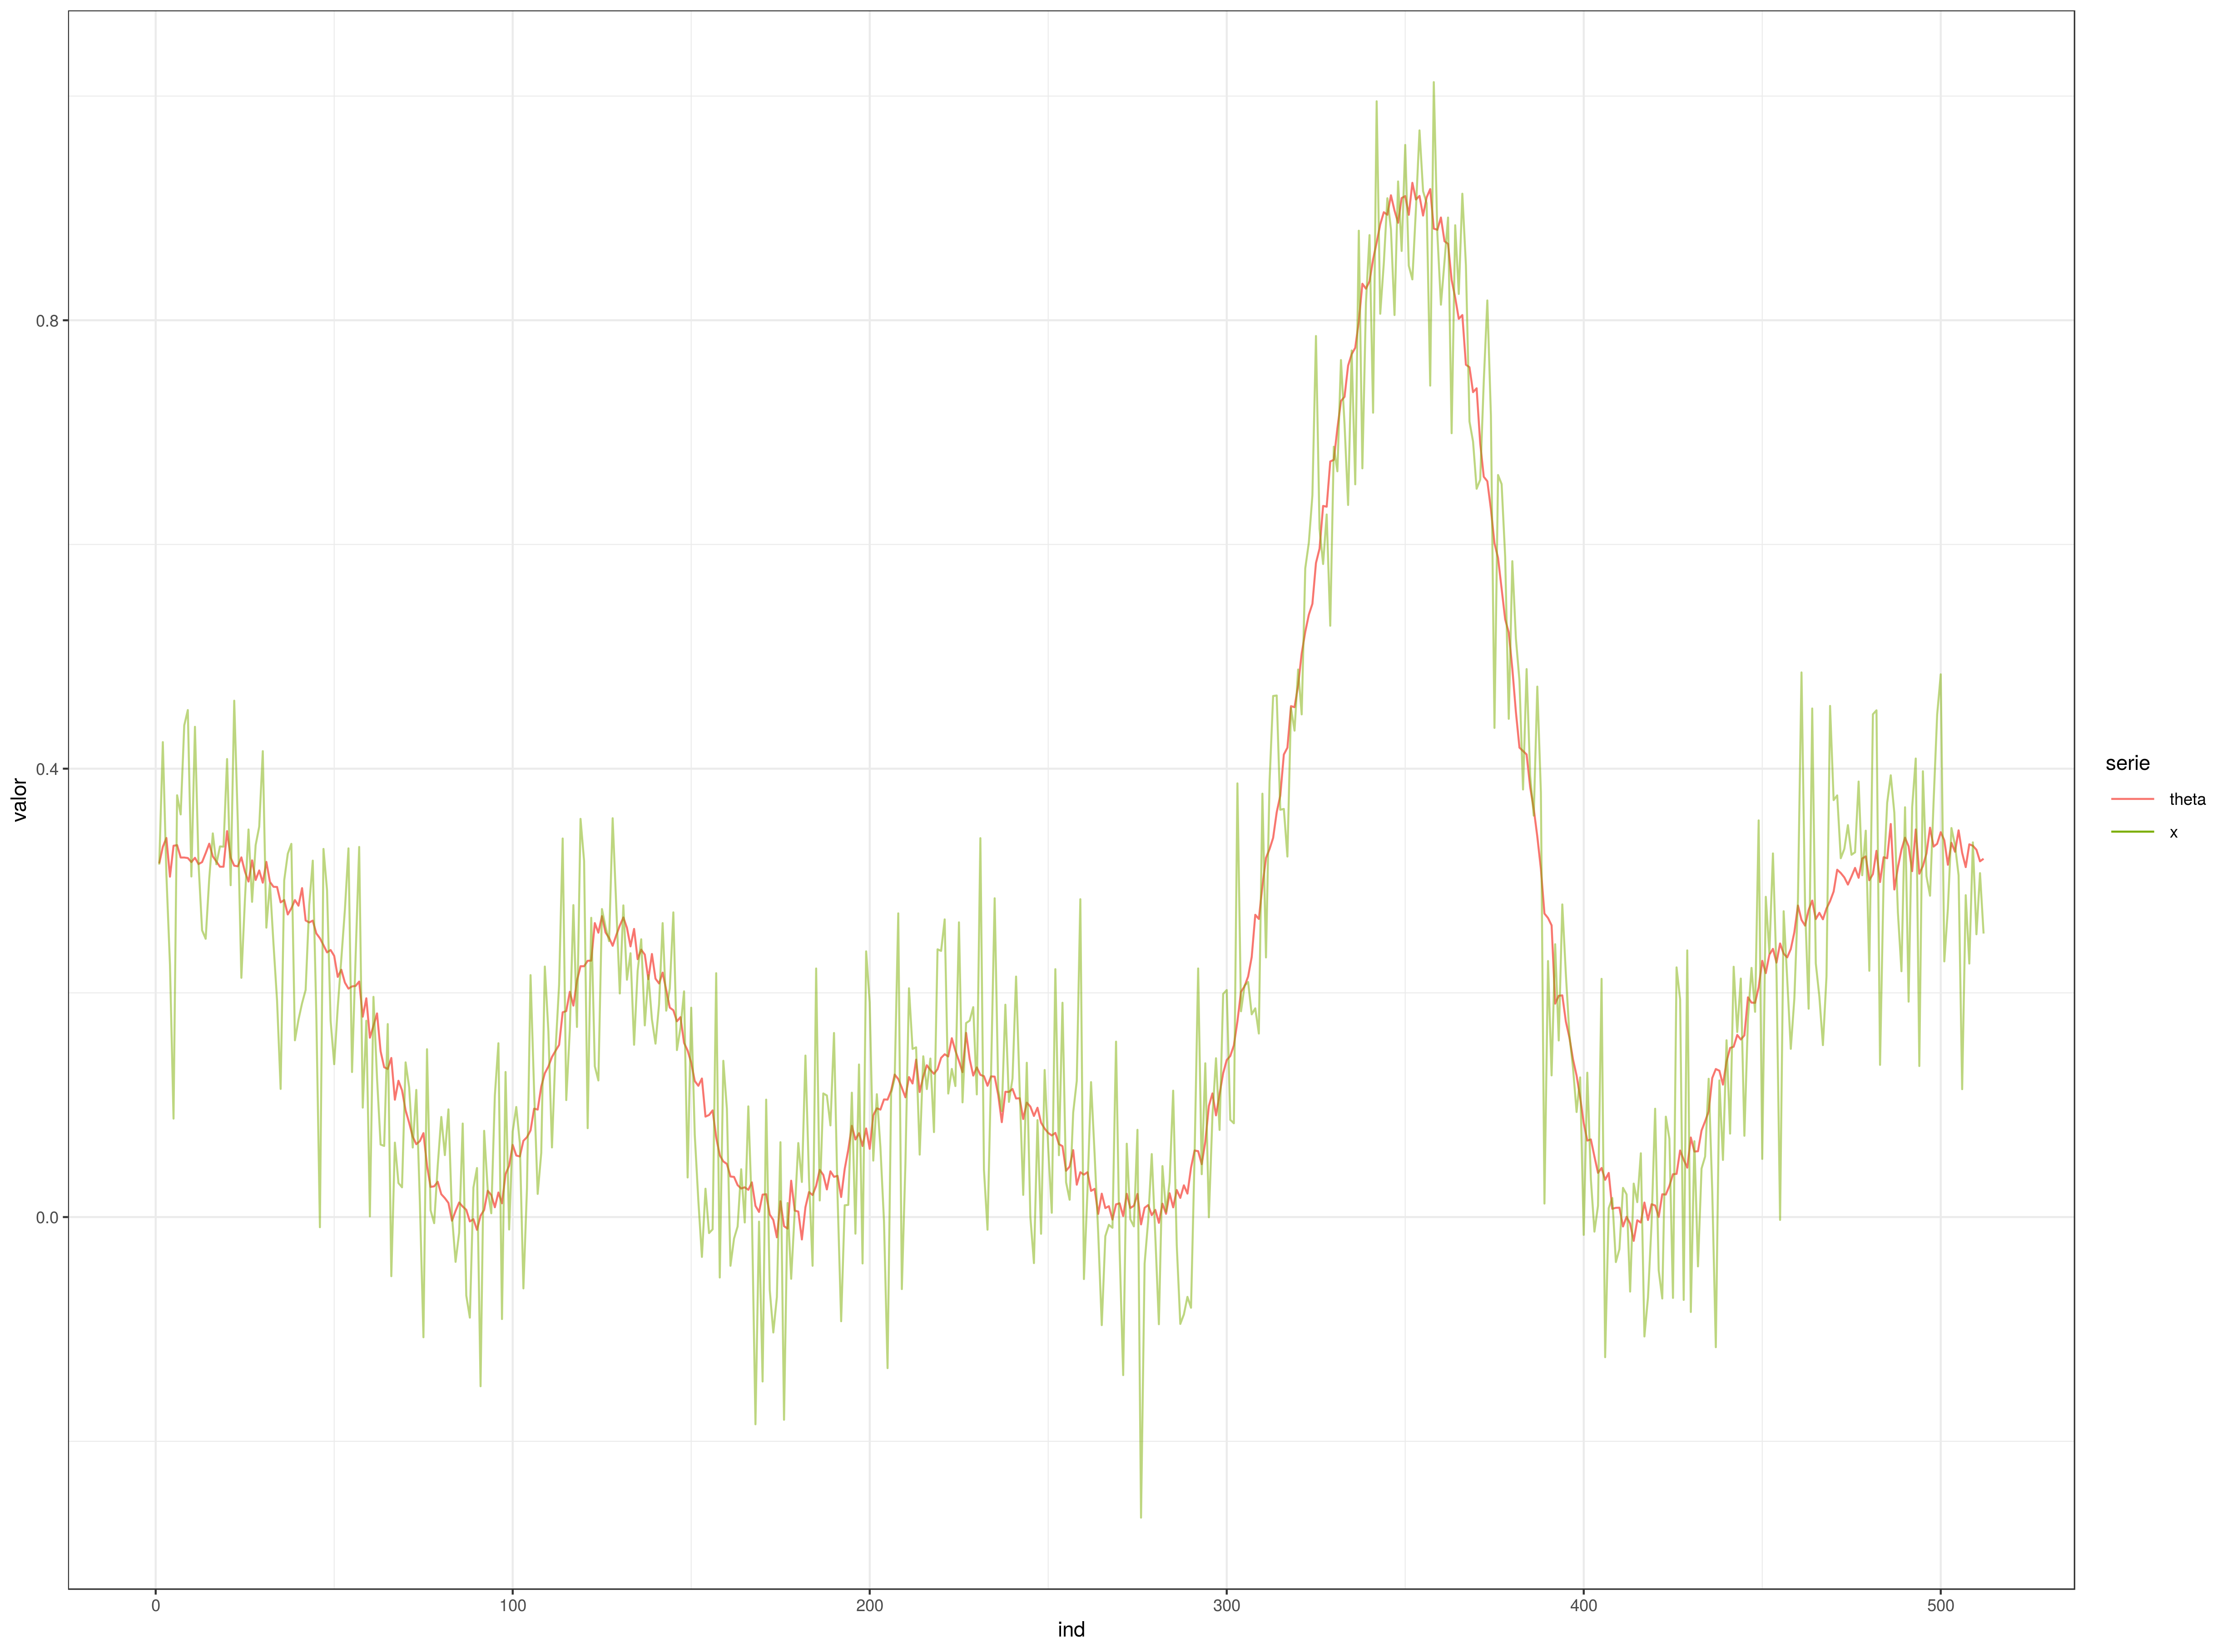
\includegraphics[width=.45\textwidth ,height=12em]{graf7.png}
\vspace{-.75em}
\captionof{figure}{Ejemplo de un proceso de espacio de estado. En rojo, se representa el proceso \textit{no-observable}, en verde se representa su observación.}
\label{fig:graf7}
\end{center}

\section{DLM estacional para las temperaturas}

Modelaremos la serie de mínimas y máximas de forma independiente, utilizaremos el mismo modelo para ambas.

Dada la fuerte característica estacional de los datos de temperaturas, es apropiado modelarla como una función periódica más un ruido aleatorio. En este caso, el proceso latente será modelado como una función periódica de período 365 y su dinámica no será aleatoria, esto se traduce en imponer matrices de varianza nulas para la ecuación de evolución.
Tal función está caracterizada por un vector $\alpha \in \RR^{365}$, la representación de $\alpha$ en la base canónica nos habla de su naturaleza temporal -\textit{qué temperatura esperamos cada día del año}-. Será de mayor interés trabajar con su representación en series de Fourier. Esto nos permitirá trabajar en un espacio de dimensión significativamente menor, con muy poca pérdida de información, dado que unos pocos armónicos (en nuestro caso 2) tienen coeficientes de fourier `significativos', definiendo así un criterio para descartar armónicos de mayor frecuencia, responsables de la rugosidad de la serie.

En este caso el modelo será:
$$\theta_t=\left(\begin{array}{lr}
S_1:=& a_1\cos\left(\frac{2\pi t}{365}\right) + b_1 \sin\left(\frac{2\pi t}{365}\right) \\
S_1^*:=& -a_1\sin\left(\frac{2\pi t}{365}\right) + b_1 \cos\left(\frac{2\pi t}{365}\right) \\
S_2:= &a_2\cos\left(\frac{4\pi t}{365}\right) + b_2 \sin\left(\frac{4\pi t}{365}\right) \\
S_2^*:=& -a_2\sin\left(\frac{4\pi t}{365}\right) + b_2 \cos\left(\frac{4\pi t}{365}\right) \\
\end{array}\right)\; F_t=(1,0,1,0) \; \forall \, t$$

La matriz $G_t$ (constante en $t$) será una matriz diagonal por bloques, cuyos dos bloques serán matrices de rotación de ángulos horarios $\frac{2\pi}{365}$ y $\frac{4\pi}{365}$. La matriz $W_t$ se definió nula. La varianza observacional $V_t$ será estimada por máxima verosimilitud.

\begin{center}
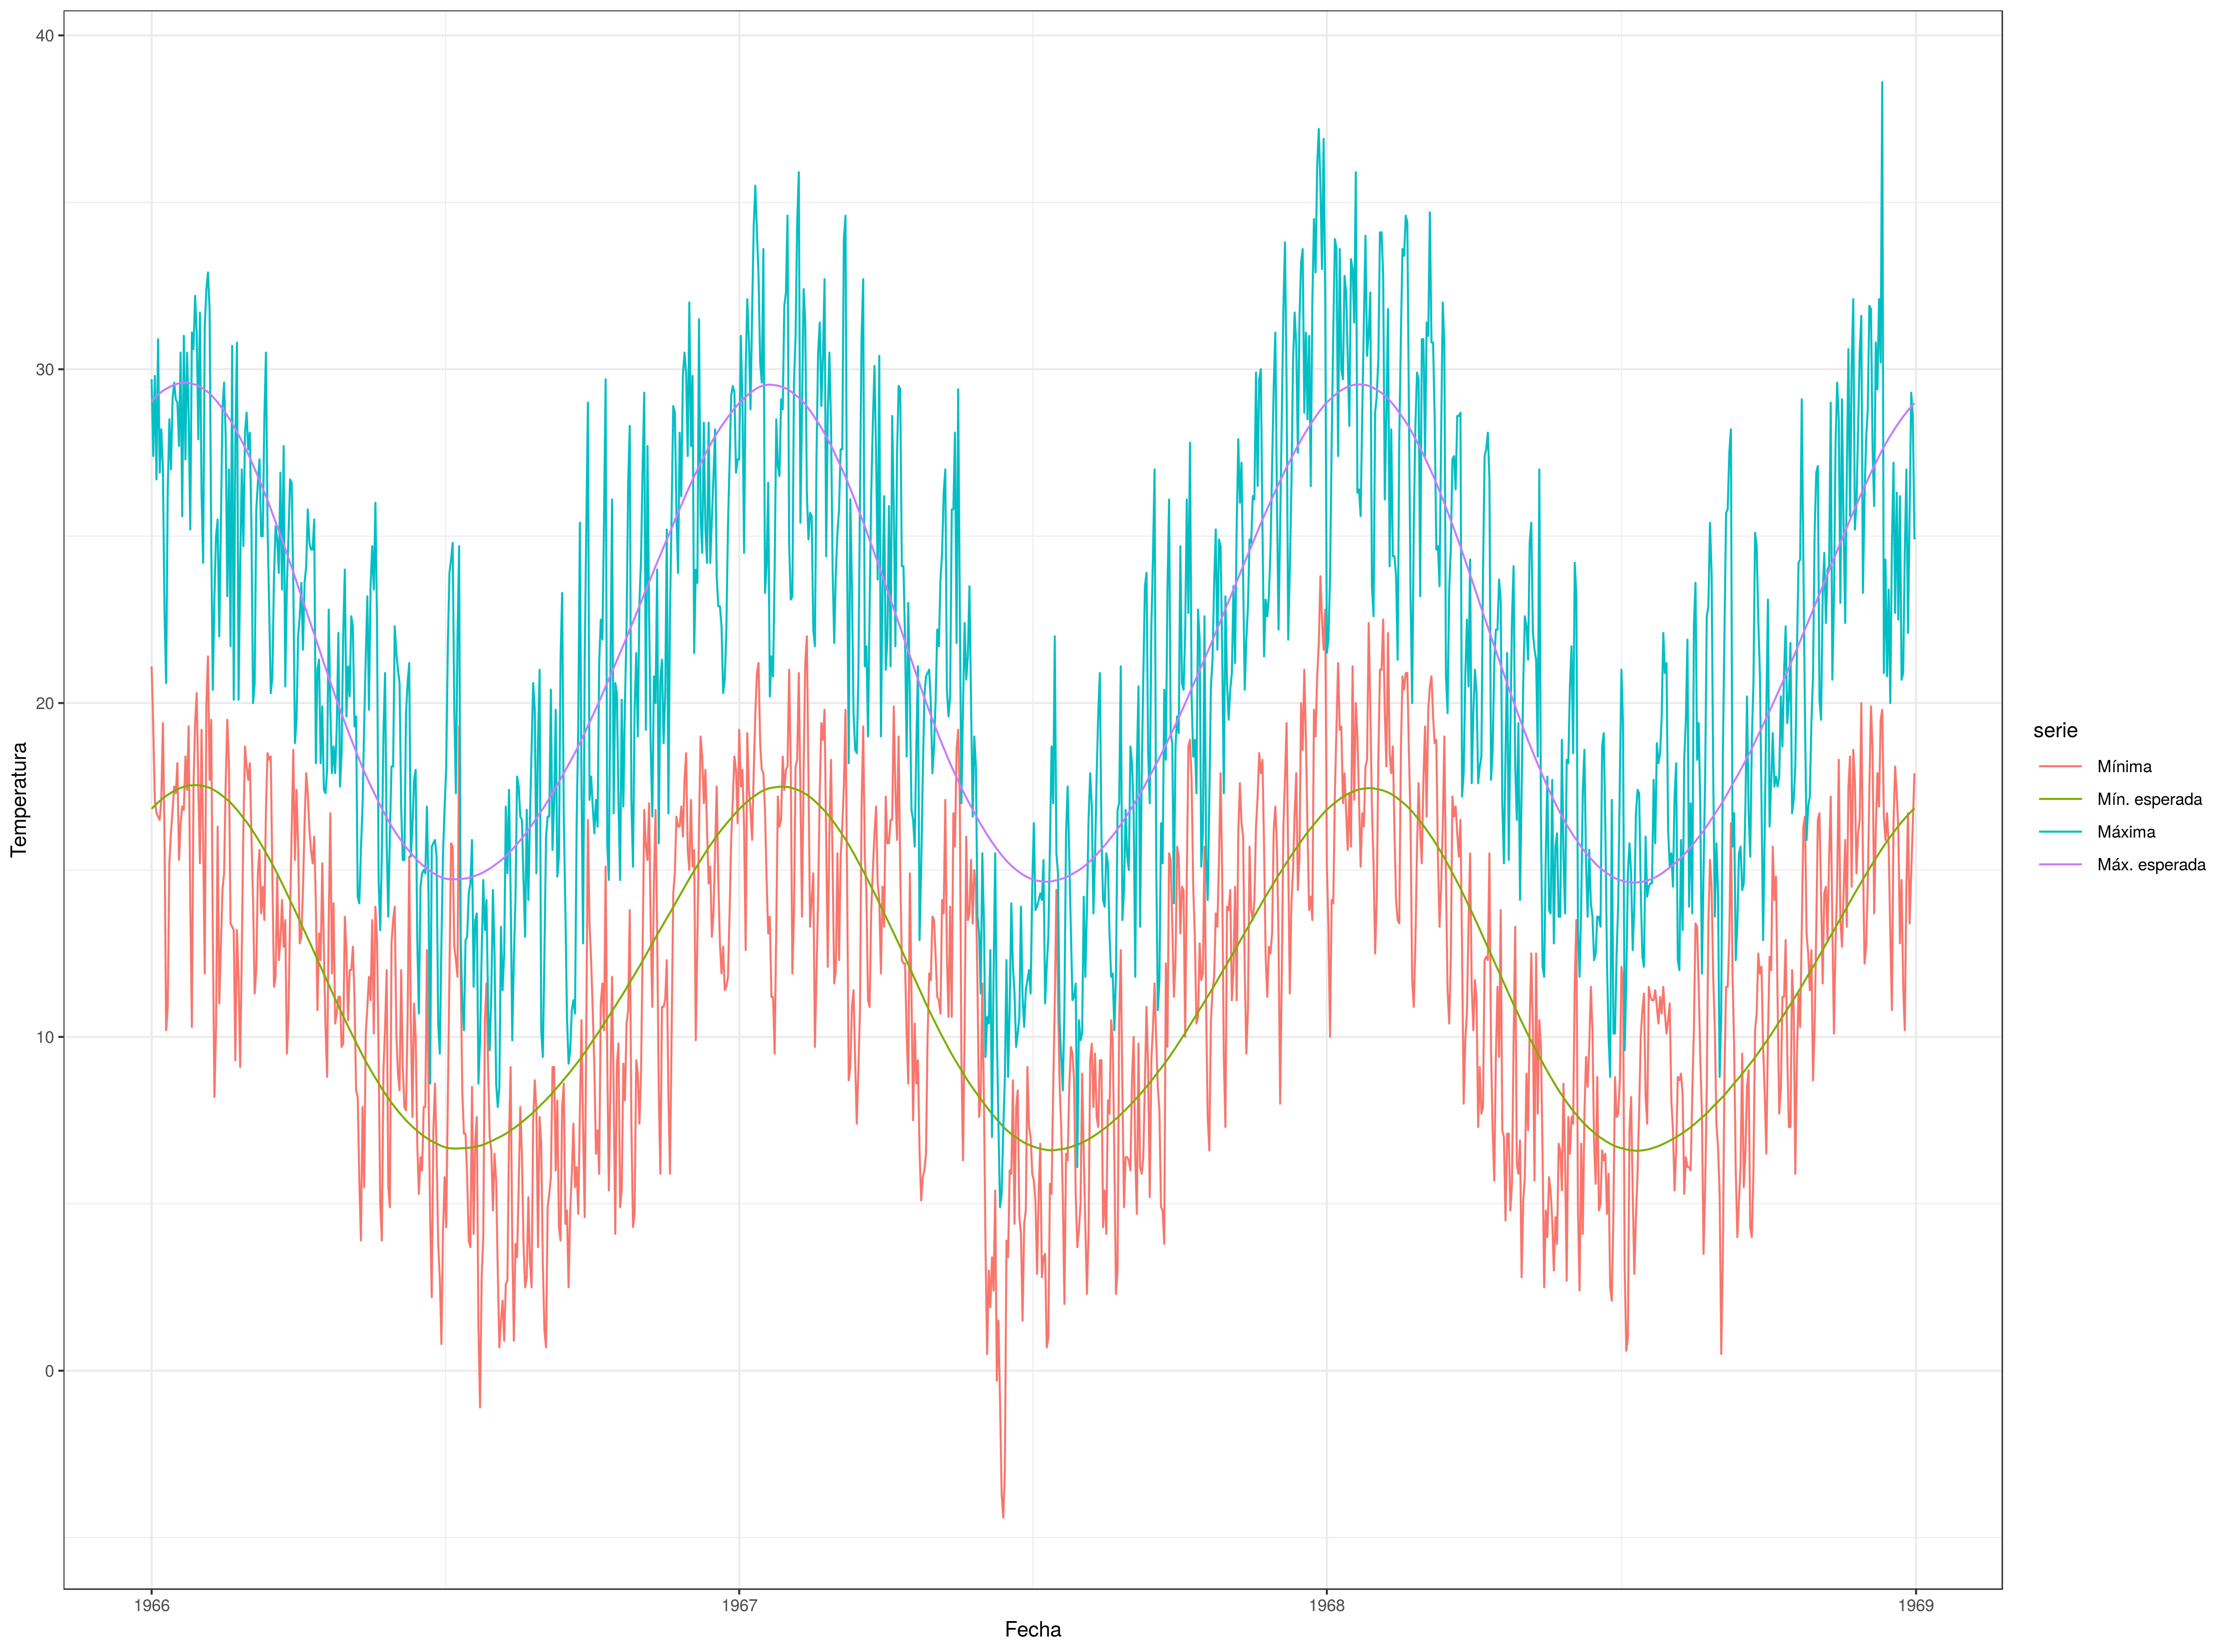
\includegraphics[width=.45\textwidth ,height=15em]{graf6.png}
\vspace{-.75em}
\captionof{figure}{Gráfico de mínimas y máximas del 1966 al 1969, y la estimación del valor esperado del proceso, mediante el filtro de Kalman}
\label{fig:graf6}
\end{center}


\section{Implementación en R - paquete `dlm'}

El paquete \verb|dlm| permite trabajar con toda la familia de modelos lineales dinámicos. %La función \verb|dlmMoTrig| nos permite crear objetos \verb|dlm| de 

Si el objeto \verb|y| contiene una de las series de temperaturas, el siguiente programa nos dará la estimación del modelo.

Lo primero es estimar la varianza observacional con la función \verb|dlmMLE|, que aproximará una estimación óptima, con un algoritmo iterativo. Para ello, primero debemos crear una función auxiliar (\verb|parMLE|), cuyo argumento sea un valor inicial propuesto para el parámetro, que retorne un objeto de la clase \verb|dlm|, en este caso de la familia de modelos trigonométricos, donde la frecuencia es 365. Le especificamos que mantenga 2 armónicos y descarte el resto:\\
\verb|parMLE <- function(par)  dlmModTrig(s = 365,q=2, dV = par, dW = 0)|

La función \verb|dlmMLE| devolverá el modelo, con el/los parámetros estimados:\\
\verb|mod<- dlmMLE(y,parm = 16,build= parMLE)|

Una vez estimado el modelo, podemos aplicar el filtro de Kalman (\verb|dlmFilter|) para obtener estimaciones de la esperanza \textit{a posteriori}:\\
\verb|Tn.filter <- dlmFilter(y,parMLE(mod$par))|

En la figura \ref{fig:graf6} se muestra en un período de tres años, las series de mínima y máxima y la estimación de su valor esperado mediante el filtro de Kalman.

\section{Estimación de percentiles}

Como se explicó anteriormente, para caracterizar olas de frío debemos estimar los percentiles 10 de temperaturas mínimas y máximas para cada día del año. Tenemos las series temporales de los datos de mínima y máxima, a escala diaria, desde el 1-Enero de 1950 hasta el 10-Octubre de 2014, por tanto para cada día del año (del 1-Enero al 31-Diciembre) tenemos más de sesenta observaciones de temperaturas. Esto da para cada día del año una distribución de temperaturas.  %Un acercamiento a este problema se puede ver en {\color{red}[referencia a Santiago]} donde se computa el percentil empírico para cada día del año y luego, a la serie de percentiles, se le aplica un filtro de medias móviles con una ventana de 31 días para obtener una estimación suave.

En este trabajo, para la estimación de tales percentiles, nos valdremos de que en el modelo descripto en la expresión (\ref{eq:modelo}) se cumple $\theta_t | \{y_1,\dots,y_t\} \sim \mathcal{N}(m_t,C_t)$, y $y_t|\theta_t \sim \mathcal{N}(Fm_t,FC_tF^T + \text{v}_t)$. El filtro de Kalman nos devuelve las secuencias $(m_t)_{1\leq t \leq T}$ y $(C_t)_{1\leq t \leq T}$ para la serie de temperaturas mínimas y máximas. Por tanto el estimador para el percentil 10 de mínima para el día $t$ será $\hat{p}^n_{10_t}:=Fm_t+\sqrt{FC_tF^T + \text{v}_t}\times z_{0.10}$. Análogamente se hizo lo mismo para el percentil 10 de las máximas.

\begin{center}
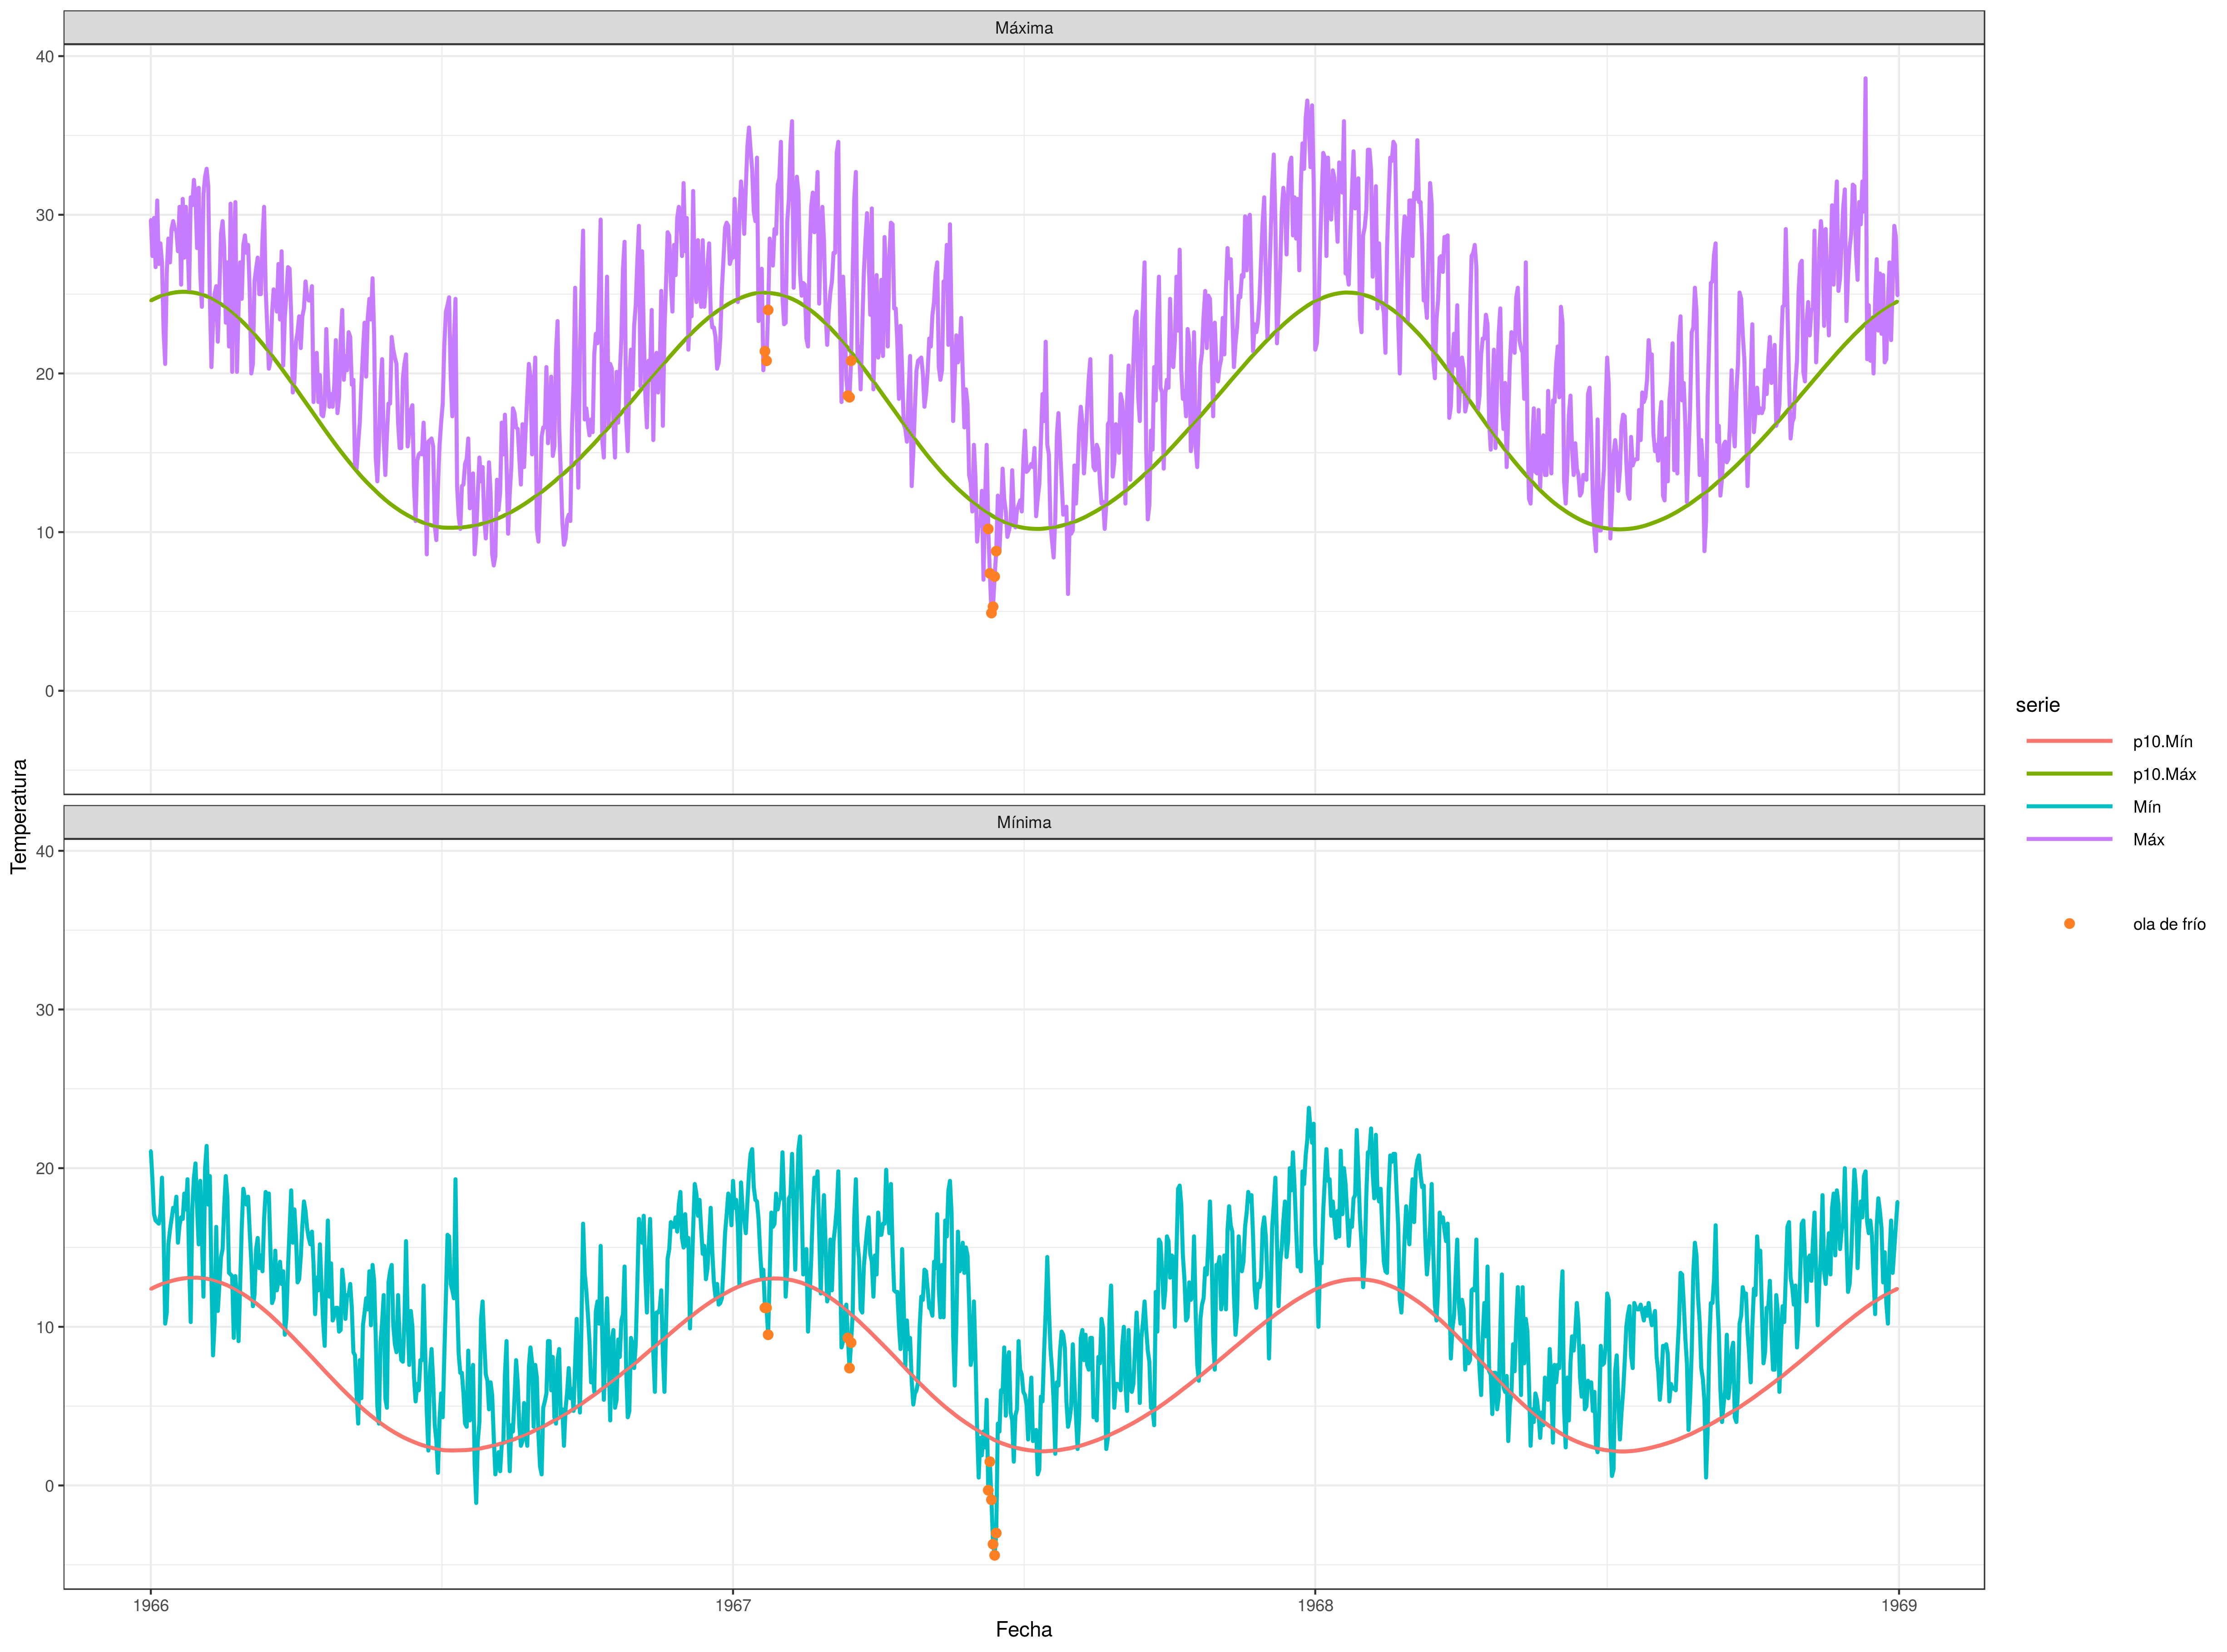
\includegraphics[width=.4\textwidth,height=21em]{graf4.png}
\captionof{figure}{Mínimas y máximas del 1966 al 1969, percentiles 10, y olas de frío detectadas}
\label{fig:graf4}
\end{center}

\begin{scriptsize}
\begin{center}
\begin{tabular}{lrrrr}
  \hline
Fecha & Mín & Máx & p10 mín & p10 máx \\ 
  \hline
1967-06-09 & 5.40 & 3.14 & 15.50 & 11.25 \\ 
  1967-06-10 & -0.30 & 3.08 & 10.20 & 11.19 \\ 
  1967-06-11 & 1.50 & 3.03 & 7.40 & 11.12 \\ 
  1967-06-12 & -0.90 & 2.97 & 4.90 & 11.06 \\ 
  1967-06-13 & -3.70 & 2.92 & 5.30 & 11.00 \\ 
  1967-06-14 & -4.40 & 2.86 & 7.20 & 10.94 \\ 
  1967-06-15 & -3.00 & 2.81 & 8.80 & 10.88 \\ 
  1967-06-16 & 3.90 & 2.77 & 12.30 & 10.83 \\ 
   \hline
\end{tabular}
\captionof{table}{Mínimas, máximas y percentiles 10 de mínimas y máximas, en ocasión de ola de frío detectada, desde el 10 al 16 de junio de 1967, }
\end{center}
\end{scriptsize}

\section{Referencias}

\begin{itemize}
\item Petris, G., Petrone, S., \& Campagnoli, P. (2009). Dynamic linear models. In Dynamic Linear Models with R (pp. 31-84). Springer, New York, NY.

\item Niemi, J. (2012). STAT 615: Advanced Bayesian Methods [Beamer slides]. Retrieved from http://www.jarad.me/courses/stat615/slides/DLMs/DLMs.pdf

\end{itemize}



\end{document}